\subsection{Creating a project}
\begin{itemize}
	\item{Navigate to project list page}
	\newline
	After you have signed in you will be navigated to the projects list page, if you are navigating there from another page, you can simply click on the projects tab on the left side navigation bar.
	\begin{figure}[H]
	    	\centering
	    	\fbox{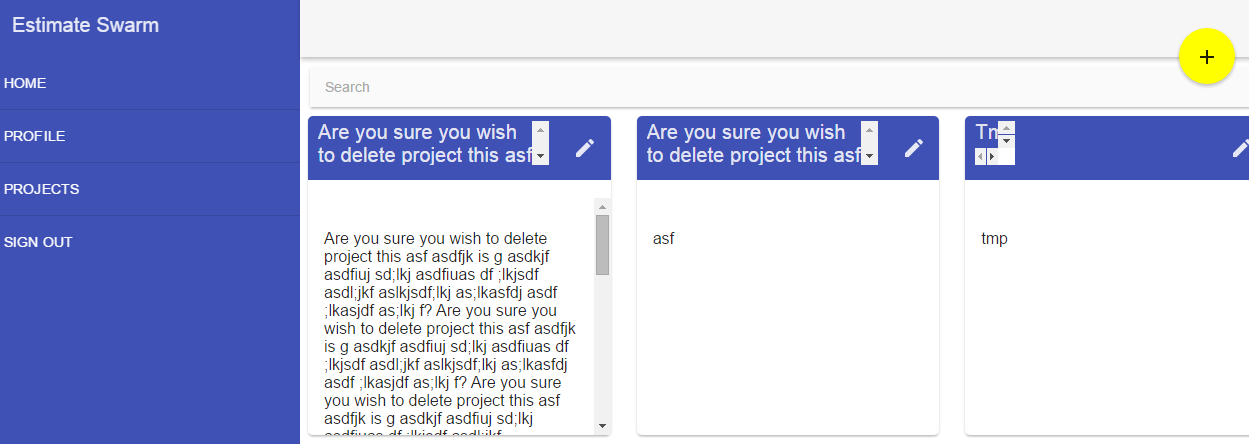
\includegraphics[width=0.5\textwidth]{projectsList}}
	    	\caption{Projects List Page}
	    	\label{fig:Learning rate 0.1}
   	\end{figure}
	\item{Add a new project}
	\newline
	On the project list page, you can simply click on the "add project" button that is in the top right hand corner of the screen.
	\begin{figure}[H]
	    	\centering
	    	\fbox{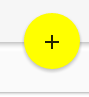
\includegraphics[width=0.5\textwidth]{addButton}}
	    	\caption{Add Project Button}
	    	\label{fig:Learning rate 0.1}
   	\end{figure}
	\item{Complete details of the project}
	\newline
	On the "Create Project" page you will have to fill in the details of the project in order to complete the creation of the project. You will have to give the project a name and a description. You will also have to indicate who will be allowed to estimate on the project as shown in the figure below.
	\begin{figure}[H]
	    	\centering
	    	\fbox{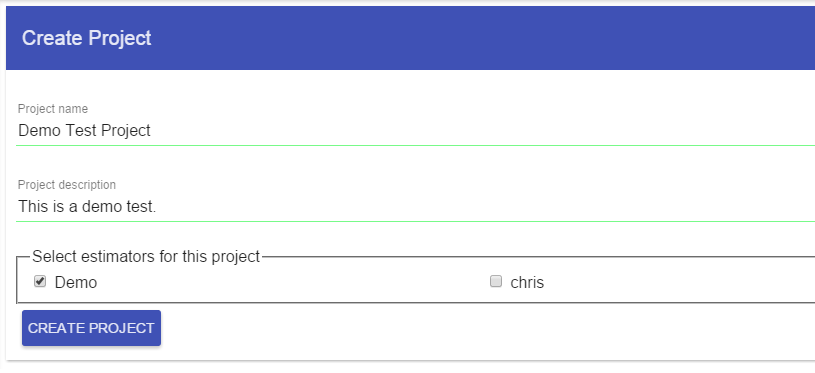
\includegraphics[width=0.5\textwidth]{createProj}}
	    	\caption{Create Project Page}
	    	\label{fig:Learning rate 0.1}
   	\end{figure}
\end{itemize}
\subsection{Estimation Process}
\begin{itemize}
	\item{Create Project Tree}
	\newline
	From here you will have to create a project tree that represent the project that you need an estimation on. You can do this by adding nodes, by clicking on the "Add node" buttons, to the project tree and naming them appropriately. You can save the tree by clicking on the "Save Project" button to continue editing the tree at a later point. When you are satisfied with the tree, you can open it for estimation, by clicking on the "Open For Estimation" button. After the project has been opened for estimation, it can not be edited again. Emails will be sent out the users that were chosen to estimate on the project to inform them that the project is now available for estimation.
	\begin{figure}[H]
	    	\centering
	    	\fbox{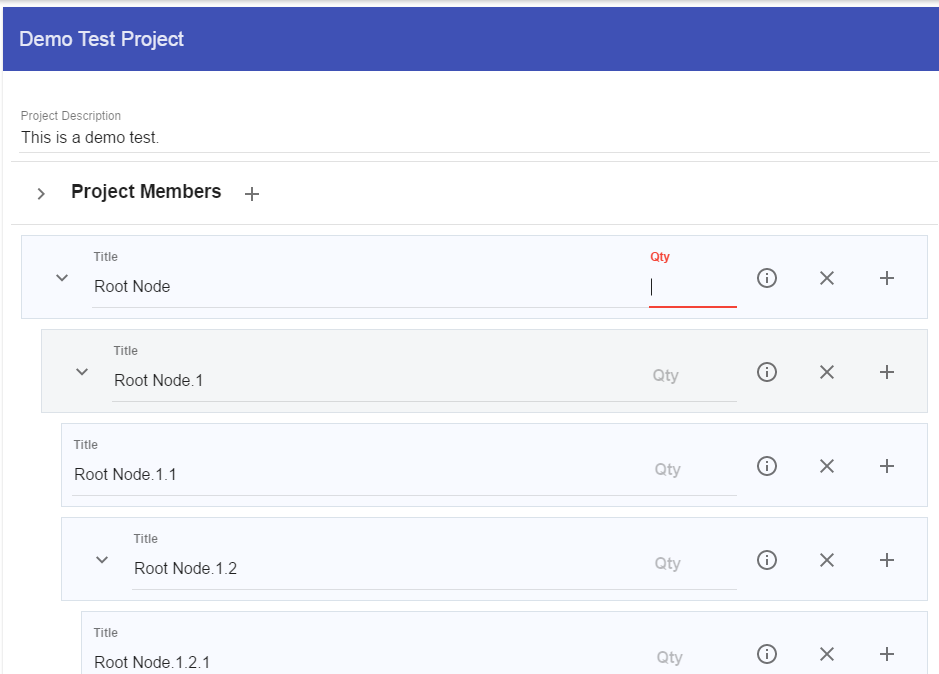
\includegraphics[width=0.5\textwidth]{createTree}}
	    	\caption{Create Tree Page}
	    	\label{fig:Learning rate 0.1}
   	\end{figure}
	\item{Estimating}
	\newline
	The estimators can nou estimate on each of the leaf nodes of the project. These values on the leaf nodes then buble up to their parent nodes, all the way up the tree to the root node. This value at the highest root node, then gives the total value of the whole tree, i.e. the total estimation that the estimator estimated on the project. When the estimator is done, he/she can click on the "Submit Estimation" button to submit his/her estimation to the project owner.
	\begin{figure}[H]
	    	\centering
	    	\fbox{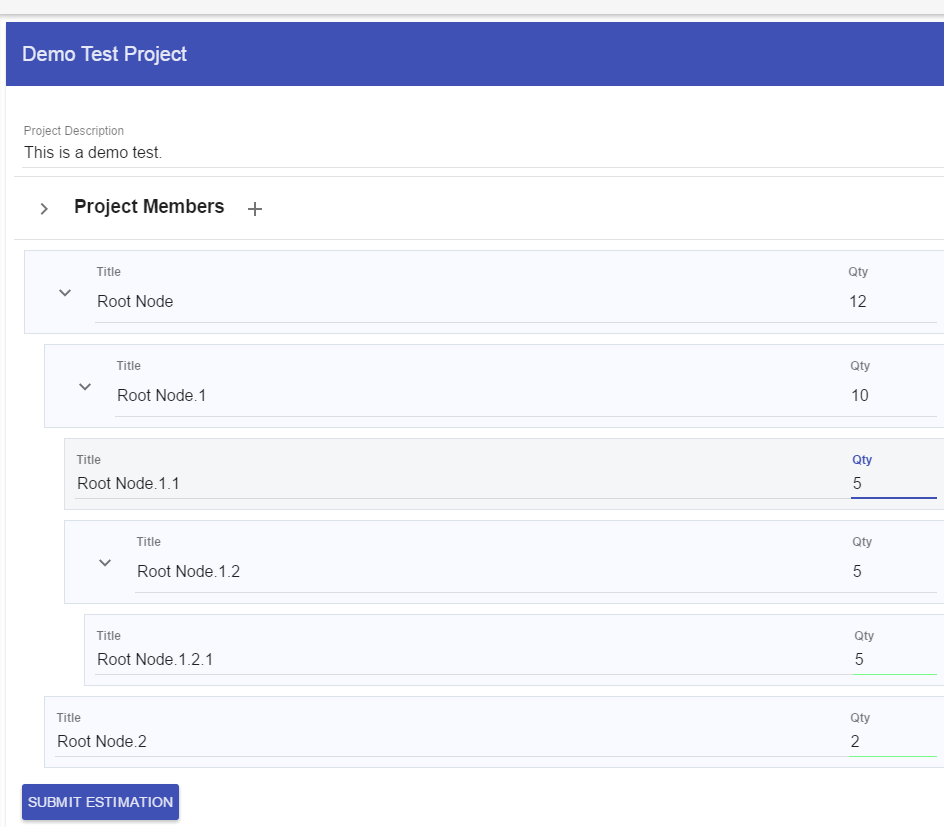
\includegraphics[width=0.5\textwidth]{estimate}}
	    	\caption{Estimation Page}
	    	\label{fig:Learning rate 0.1}
   	\end{figure}
\end{itemize}